\begin{figure}[h!]
    \footnotesize
    \begin{tabular}{@{}p{0.5\textwidth}}
Keep user posts visible to the intended audience, but anonymized by reassociation with a global
placeholder user.
\begin{lstlisting}[language=Rust]
EdgeTransforms {
  "User-Post": Retain
}
EntityTransforms {
  "User":    Gen(Default("placeholder")) 
  "Post": Copy
}
\end{lstlisting}
        \vspace{-\baselineskip}
    \\
Keep user's posts, but associate each post with a different user account.
\begin{lstlisting}[language=Rust]
EdgeTransforms {
  "User-Post": Decorrelate
}
EntityTransforms {
  "User": Gen(Random)
  "Post": Copy
}
\end{lstlisting}
        \vspace{-\baselineskip}
\\
Retain users' posts with a shared tag, but decorrelate the post 
from the tag \emph{only if} the tag was created by
the user.
\begin{lstlisting}[language=Rust]
EdgeTransforms {
  "User-Post": Decorrelate
  "Post-Tag":  Decorrelate(Filter(p.user == c.user))
}
EntityTransforms {
  "User": Gen(Random)
  "Post": Copy
  "Tag":  CopyOnce+Gen(Default(None)) 
}
\end{lstlisting}
\vspace{-\baselineskip}
        \\
Remove users' posts if they comprise more than $p$ percent of the posts
with a shared tag.
\begin{lstlisting}[language=Rust]
EdgeTransforms {
  "User-Post": Decorrelate
  "Post-Tag":  Decorrelate(Sensitivity(p))
}
EntityTransforms {
  "User": Gen(Random)
  "Post": Copy
  "Tag":  CopyOnce+Gen(Default(None)) 
}
\end{lstlisting}
\vspace{-2\baselineskip}
\end{tabular}
\caption{Example masks for a variety of privacy transformations for user posts and tags.}
\label{fig:masks}
\end{figure}

\begin{figure*}[t!]
    \centering
    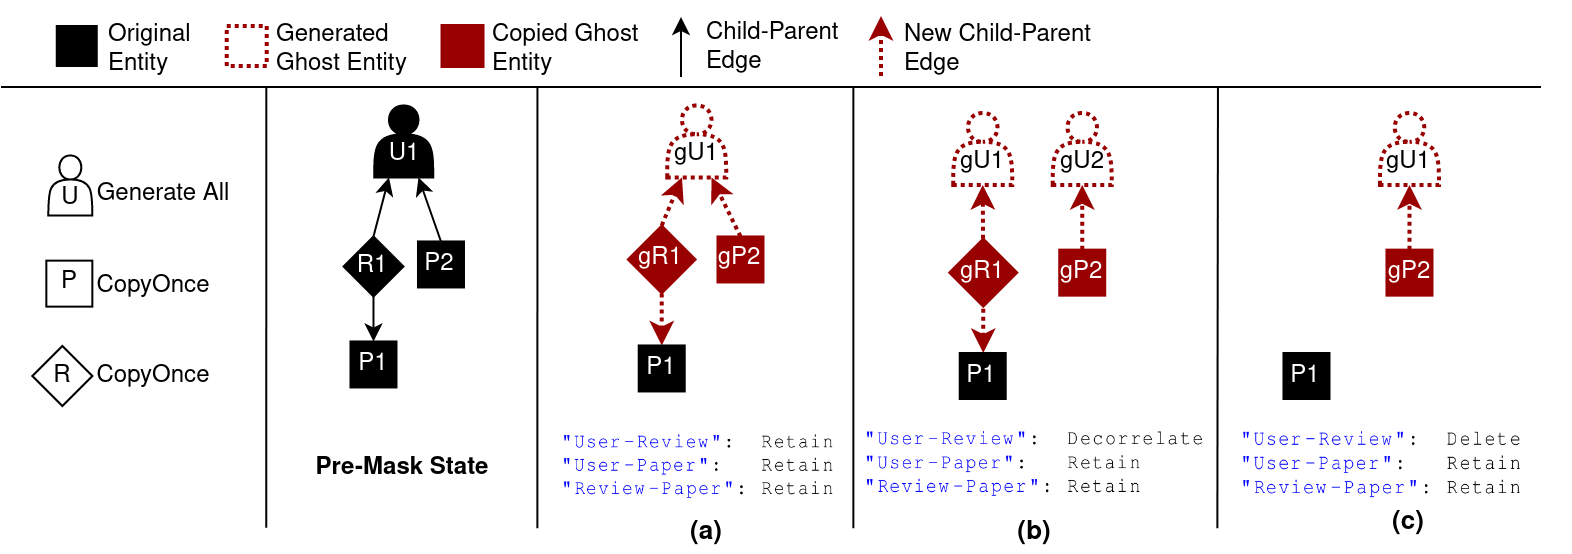
\includegraphics[width=\textwidth]{img/edge_transforms}

    \iffalse
\begin{lstlisting}[language=Rust]
"User-Review":  Retain
"User-Paper":   Retain
"Review-Paper": Retain
\end{lstlisting}

\begin{lstlisting}[language=Rust]
"User-Review":  Decorrelate
"User-Paper":   Retain
"Review-Paper": Retain
\end{lstlisting}

\begin{lstlisting}[language=Rust]
"User-Review":  Delete
"User-Paper":   Retain
"Review-Paper": Retain
\end{lstlisting}
\fi

    \caption{Different edge transformations in the entity graph. User entities are generated and
    paper and review entities are cloned once to retain their content in the application. 
    For clarity, we show only relevant parts of the entity graph and the mask policy, and use entity-granularity guises
        transformations rather than per-attribute ones.\\
    \textbf{(a)} retains User-Review edges;
    \textbf{(b)} decorrelates User-Review edges, creating a new ghost user for R1 and rewriting R1's 
    edge attribute to point to the new ghost user;
    \textbf{(c)} deletes User-Review edges.\\
    All edge transformations replace all sensitive entities (U1, R1, and P2) with ghost entities.
    }
    \label{fig:edgepol}
\end{figure*}

\begin{figure}[t!]
    \centering
    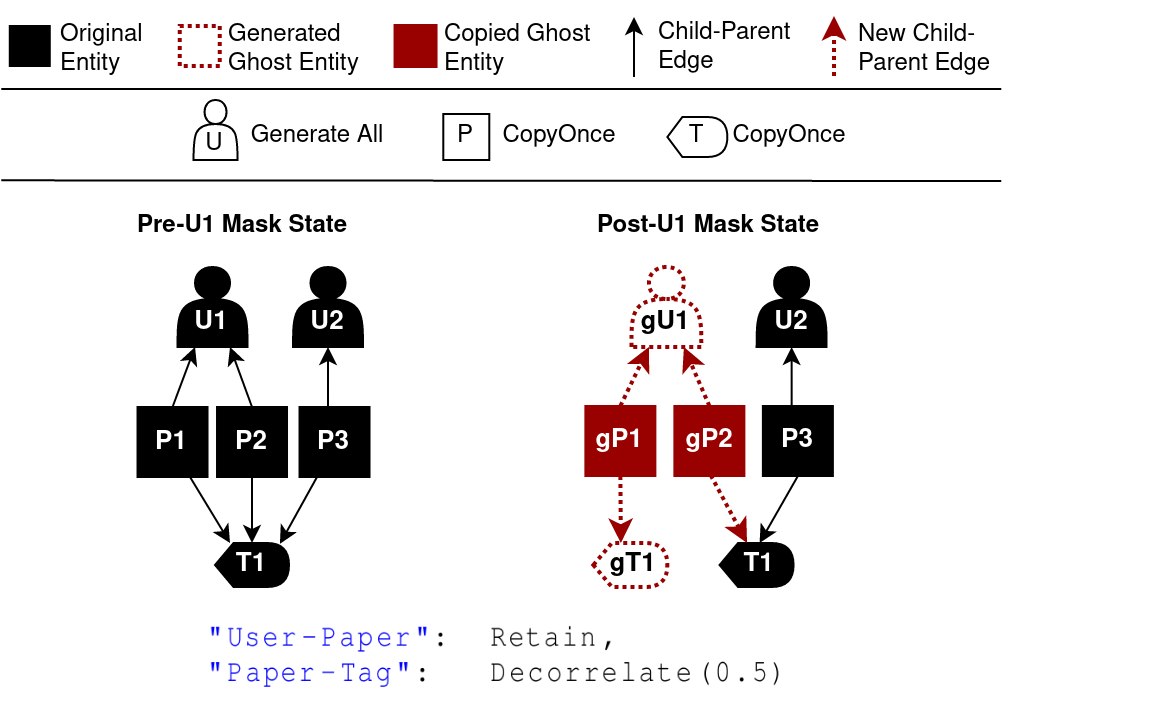
\includegraphics[width=0.55\textwidth]{img/child-parent}

    \iffalse
\begin{lstlisting}[language=Rust]
"User-Paper":  Retain,
"Paper-Tag":   Decorrelate(0.5) 
\end{lstlisting}
\fi

    \caption{An example of a decorrelation edge transformation that decorrelates papers from tags
    until at most 50\% of all papers with the tag are sensitive.
    }
    \label{fig:sensitivity}
\end{figure}


